\section{Dodatkowe informacje}
Informacje jak pisać pracę dyplomową oraz szablon pracy zostały wzięte ze strony \href{http://www.ii.pw.edu.pl/ii_pol/Instytut-Informatyki/Nauczanie/Poradnik-dyplomanta/Przygotowanie-pracy-dyplomowej}{http://www.ii.pw.edu.pl/}.

Jak wygląda proces dyplomowania w~IT można dowiedzieć się na stronie \href{https://secure.tele.pw.edu.pl/wp-content/uploads/2017/06/PROCES-DYPLOMOWANIA-17L.pdf}{https:// secure.tele.pw.edu.pl/} w~sekcji Dydaktyka > Dla studentów > Proces dyplomowania.

Aby zacytować artykuł z~Wikipedii, w~łatwy sposób można uzupełnić bibliografię o~tę pozycję. Na stronie z~wybranym artykułem np. o~\href{https://pl.wikipedia.org/wiki/LaTeX}{Latex} ależy po lewej stronie  wybrać 
\textit{Narzędzia:Cytowanie tego artykułu} i~otrzymamy gotowy 
 \href{https://pl.wikipedia.org/w/index.php?title=Specjalna:Cytuj&page=LaTeX&id=58147357}{Przypis do tej strony} \cite{Wiki:Latex}. Na innych stronach należy szukać \textit{bibtex}, \textit{cite} lub podobne.

\subsection{Rysunki}
\begin{figure}[h]
\centering
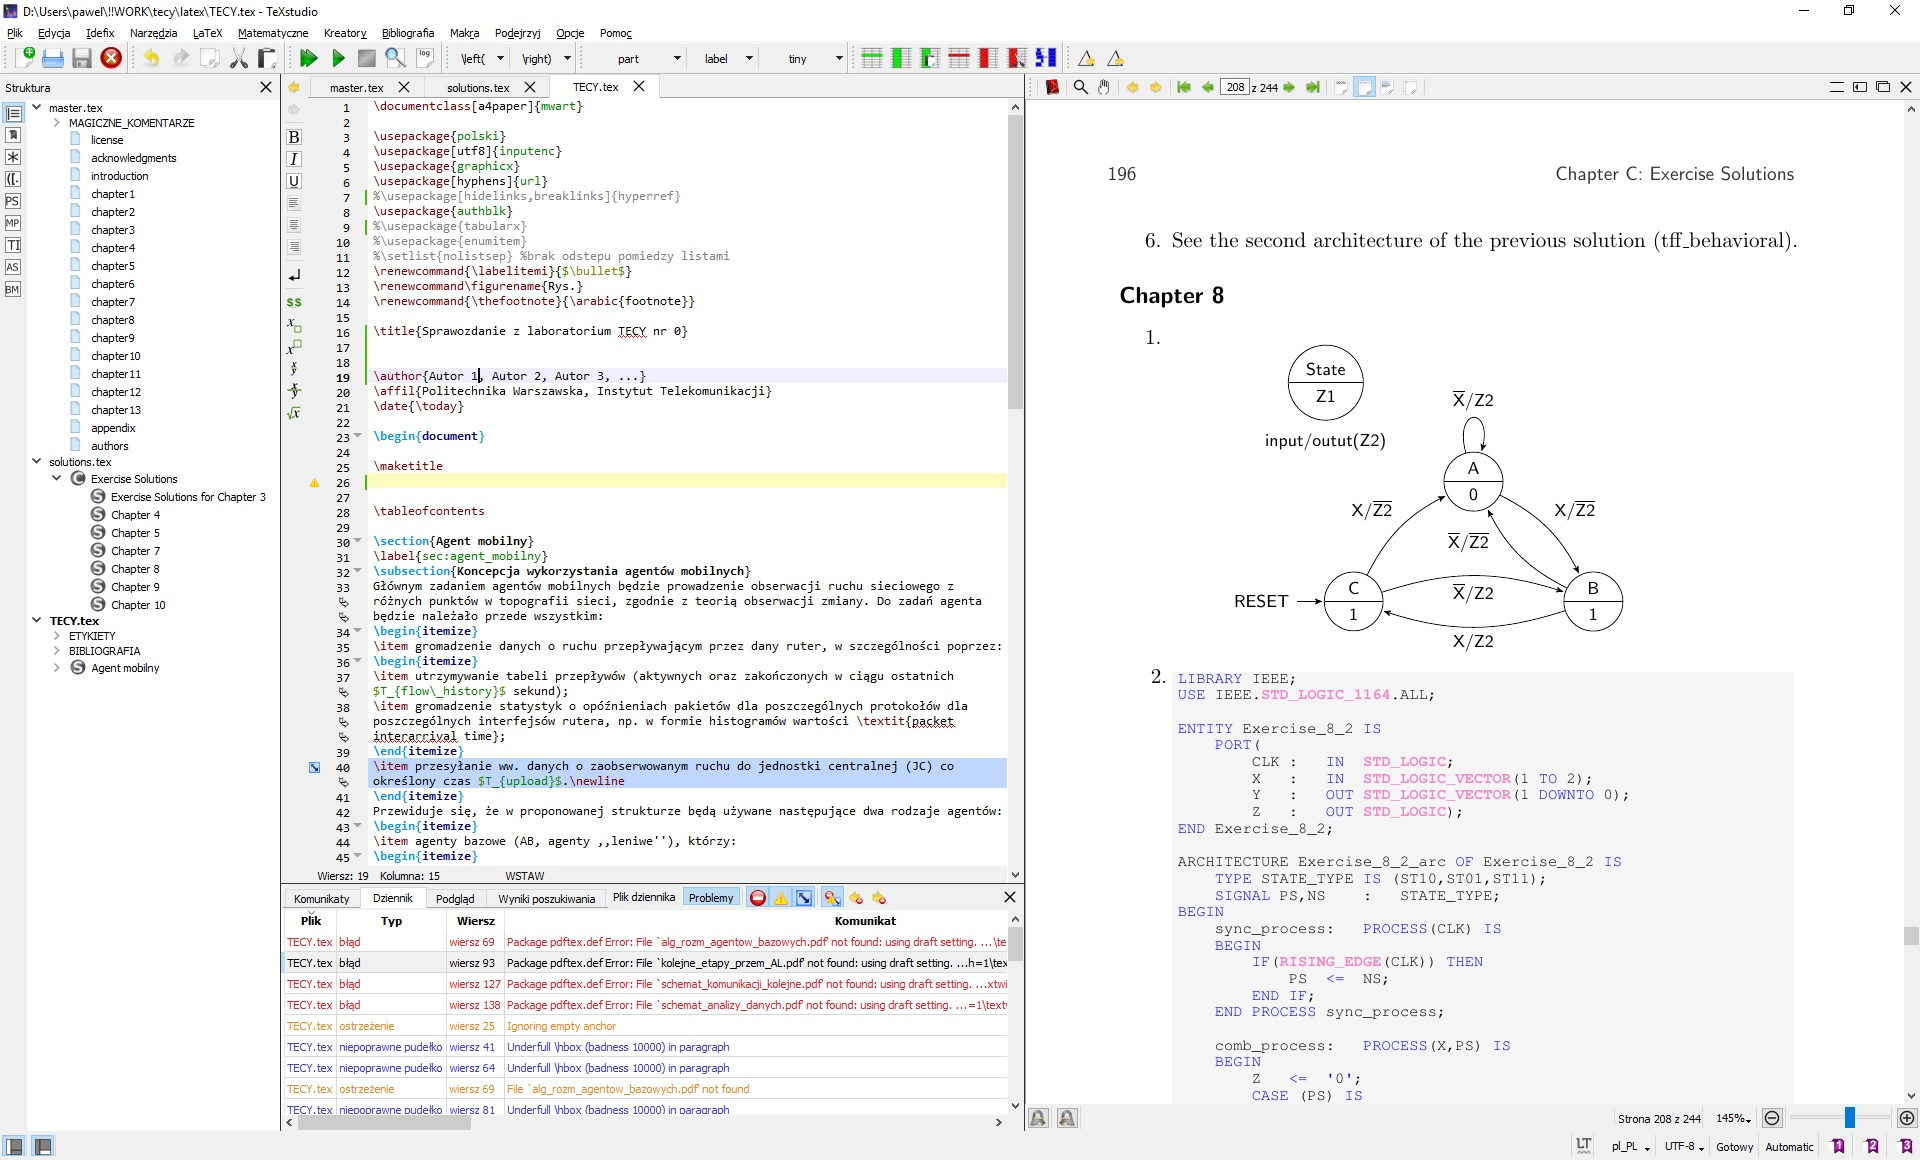
\includegraphics[width=0.5\textwidth]{rysunek_1.jpg}
\caption{\label{fig:rysunek_1}Widok edytora TeXstudio \cite{TeXstudio}}
\end{figure}
\FloatBarrier %zatrzymanie przenoszenia rysunku

\subsection{Tablice}
\begin{table}[h]
	\begin{center}
\caption{Przykładowa tabela}
\label{tab:tabela_przyklad}
\begin{tabular}{|r|l|c|c|}
	\hline 
	Miejsce & Drużyna & Gole & Punkty \\
	\hline \hline
	1 & Legia & 12 & 36 \\
	2 & Górnik & 10 & 30 \\
	3 & Widzew & 8 & 24\\
	4 & ŁKS & 7 & 21 \\ \hline
\end{tabular}
\end{center}
\end{table}
\FloatBarrier %zatrzymanie przenoszenia rysunku

\subsection{Wydruki}
\begin{lstlisting}[label=lst:wydruk,caption={Testowy program w Verilog},language=Verilog,numbers=left]
module lfsr_4 //rejestr o dlugosci 4
#(parameter n=4)
(
  input clk,
  input a_reset,
  input load,
  input [n-1:0]  a,
  output [n-1:0] result
);

reg [n-1:0] register;

always@(posedge clk, posedge a_reset)
if(a_reset)
  register <= 0;
else 
  if(load)
   register <= 1; // inicjacja
  else
   register <= {register[0],register[3:2], register[1]^register[0]};

assign result = register;

endmodule
\end{lstlisting}

\subsection{Matematyka}
Przykład użycia trybu matematycznego (poniżej).

The mass-energy equivalence is described by the famous equation

$$E=mc^2$$ %wysrodkowany bez numeracji

discovered in 1905 by Albert Einstein. 
In natural units ($c$ = 1), the formula expresses the identity %w tekscie

\begin{equation} %wysrodkowany z numeracja
E=m
\end{equation}

\subsection{Oprogramowanie - wersja Windows}
\label{sec:oprogramowanie}
Do pracy w środowisku \LaTeXe{} (wersja aktualnie używana) proponuję (wybór subiektywny i~jedynie słuszny) następujący zestaw oprogramowania \cite{Ghostscript, MikTeX, TeXstudio}, instalacja w takiej kolejności:
\begin{itemize}
\item Ghostscript -- interpreter plików PostScript i PDF  \url{https://www.ghostscript.com/},
\item MikTeX -- dystrybucja dla Windows  \url{https://miktex.org/} - zestaw narzędzi,
\item Adobe Reader -- przeglądarka plików PDF \url{https://acrobat.adobe.com/pl/pl/},
\item TeXstudio -- edytor i kompilator \url{https://texstudio.org/},
\item (opcjonalnie) Słownik PL do edytora -- należy zaimportować w edytorze (rys. \ref{fig:rysunek_spr})  \url{https://extensions.openoffice.org/en/project/polish-dictionary-pack},
\item (opcjonalnie) Java JRE (do uruchomienia LT) \url{https://www.java.com/pl/download/},
\item (opcjonalnie) Narzędzie Language Tool -- można uruchomić \textit{off-line} w edytorze \url{https://languagetool.org/download/LanguageTool-4.6.zip},
\end{itemize}

\begin{figure}[h]
	\centering
	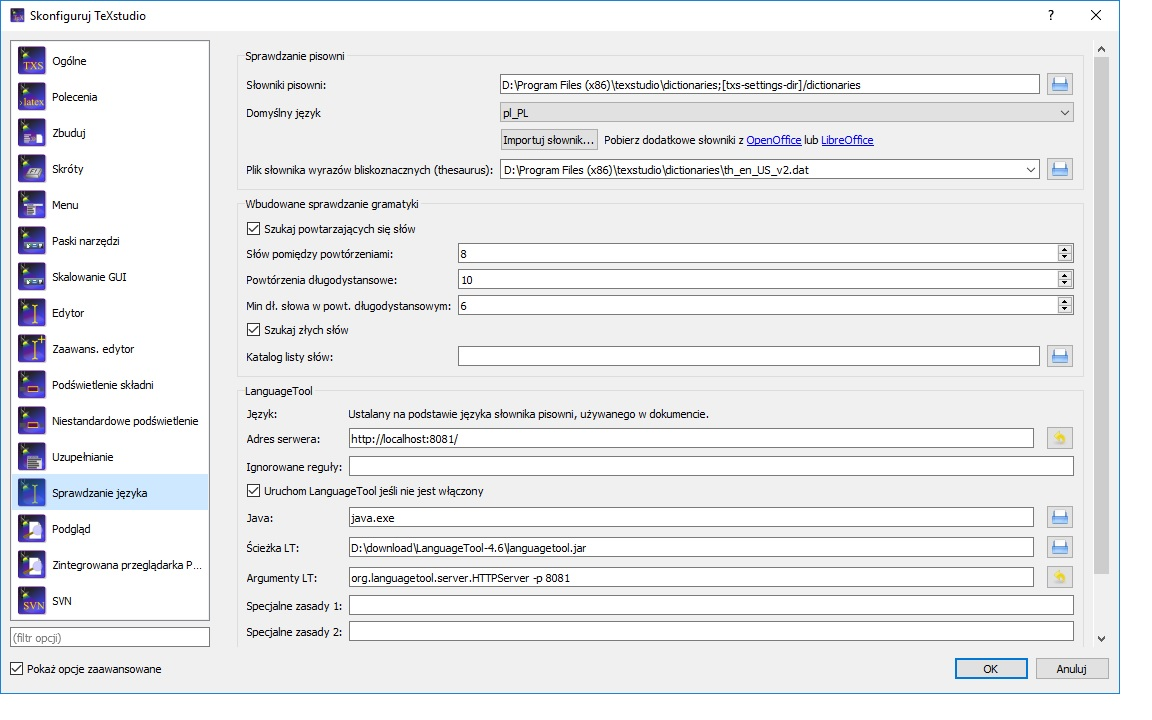
\includegraphics[width=1\textwidth]{texstudio_sprawdzanie_jezyka.jpg}
	\caption{\label{fig:rysunek_spr}Widok edytora TeXstudio -- ustawianie opcji do sprawdzania języka}
\end{figure}

Jeżeli kompilacja pierwszego dokumentu nie przebiegnie prawidłowo, tzn. kompilator nie znajdzie czcionek, należy uruchomić program \texttt{updmap.exe} z~pakietu MikTex.

Dla zawansowanych: sposób na automatyczne dodawanie tabulatora po literach a, i, o, u,w, z aby nie zostawały na końcu linii -- sierotki. Wyzwalacz \textit{trigger} ma postać \begin{verbatim}
(?language:latex)\sa\s|\si\s|\so\s|\su\s|\sw\s|\sz\s
\end{verbatim}

\begin{figure}[h]
	\centering
	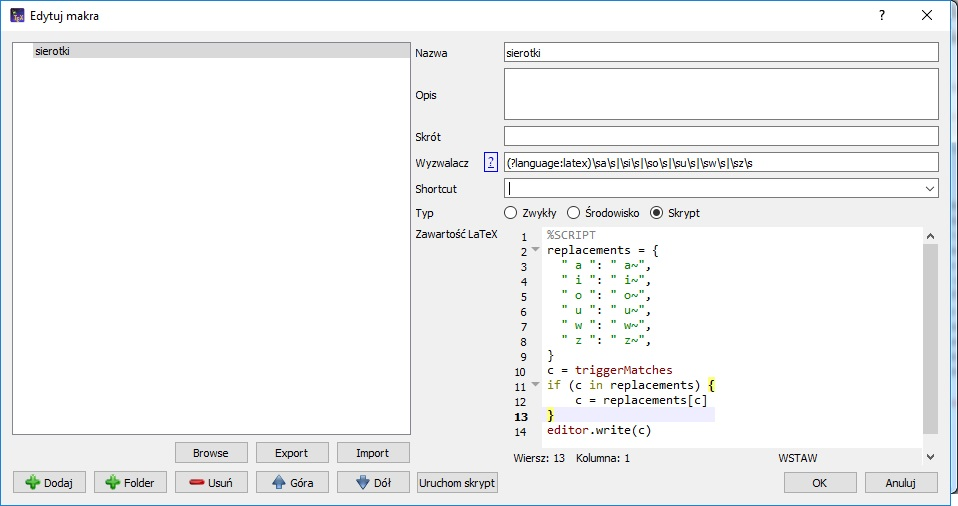
\includegraphics[width=1\textwidth]{sierotki.jpg}
	\caption{\label{fig:sierotki}Widok edytora TeXstudio -- makro dla sierotek}
\end{figure}

\begin{lstlisting}[label=lst:sierotki,caption={Widok edytora TeXstudio -- dodanie makra do sierotek},numbers=left]
%SCRIPT
replacements = {
" a ": " a~",
" i ": " i~",
" o ": " o~",
" u ": " u~",
" w ": " w~",
" z ": " z~",
}
c = triggerMatches
if (c in replacements) {
c = replacements[c]
}
editor.write(c)
\end{lstlisting}


\subsection{Inne strony}
\begin{itemize}
\item Obowiązkowa lektura: \url{ftp://ftp.gust.org.pl/TeX/info/lshort/polish/lshort2e.pdf}	
\item \url{http://www.mif.pg.gda.pl/homepages/sylas/students/wdi/index.html},
\item \url{https://www.mimuw.edu.pl/~mbodnar/prosem/wprowadzenie_v2016.pdf}	
\item \url{http://latex-kurs.x25.pl//}
\item \url{https://matematyka.pl/viewtopic.php?t=28951}	
\item \url{https://pl.wikibooks.org/wiki/LaTeX}	
\item \url{https://en.wikibooks.org/wiki/LaTeX}
\item Edytor i kompilator \textit{on-line} Overleaf -- także do pracy grupowej \url{https://www.overleaf.com/}
\item \url{https://www.google.com/search?q=latex+tutorial+pl} \dots	
\end{itemize}
